\section{Chirality and Chiroptical Effects}
\label{sec:background:ChiropticalEffects}

\subsection{Chirality}
\label{sec:chirality}

Chirality is an important property pervasive throughout nature, found in organic chemistry, and hence key to biological organisms~\cite{Berova2012}, as well as throughout physics in systems such as spiral galaxies, fluid vortices, and particle angular momentum to name just a few. Chirality is also frequently encountered in photonics, though chiral electromagnetic fields. At its simplest, this manifests as the circular polarisation of light. Here, two orthogonal linearly polarised waves of equal amplitude, wave vector and frequency, but with a relative phase shift of $\pm \pi/2$ are superimposed (Figure~\ref{fig:test_include:test_figure}). The sign of this phase shift determines the handedness of circularly polarised light (CPL), with the wave equations for left-circularly polarised (LCP) and right-circularly polarised (RCP) given by equation~\ref{eq:chirality:CPL}~\cite[\S 8.1.2]{Hecht2013}).
\begin{equation}
    \label{eq:chirality:CPL}
    \begin{split}
        & \mathbf{E}_{RCP} = E_0 \left[ \mathbf{\hat{x}} \cos(\mathbf{k} z-\omega t) + \mathbf{\hat{y}} \sin(\mathbf{k} z-\omega t )\right]\\
        & \mathbf{E}_{LCP}= E_0 \left[ \mathbf{\hat{x}} \cos(\mathbf{k} z-\omega t) - \mathbf{\hat{y}} \sin(\mathbf{k} z-\omega t )\right]
    \end{split}
\end{equation}

Due to the abundance of chiral molecules in organic chemistry, biology, and pharmacology, there is a growing emphasis on the importance of accurate, sensitive, and accessible characterisation of such molecules. The use of chiral light in sensing applications has become an active field of current research, due to the flexibility of chiral photonics. However, a common fundamental mechanism exploited is chiral dissymmetry in the excitation of molecules. If a molecule couples differently to one circular polarisation than the other, it will experience a chiral dissymmetry in rate or phase of excitation, equivalent to a difference in the complex refractive index of the molecular material between LCP and RCP. This difference in excitation rate and phase delay results in measurable circular dichroism (CD) and optical rotation (OR)~\cite[\S 1]{purdie1993}.

\begin{figure}[htb!]
    \centering
    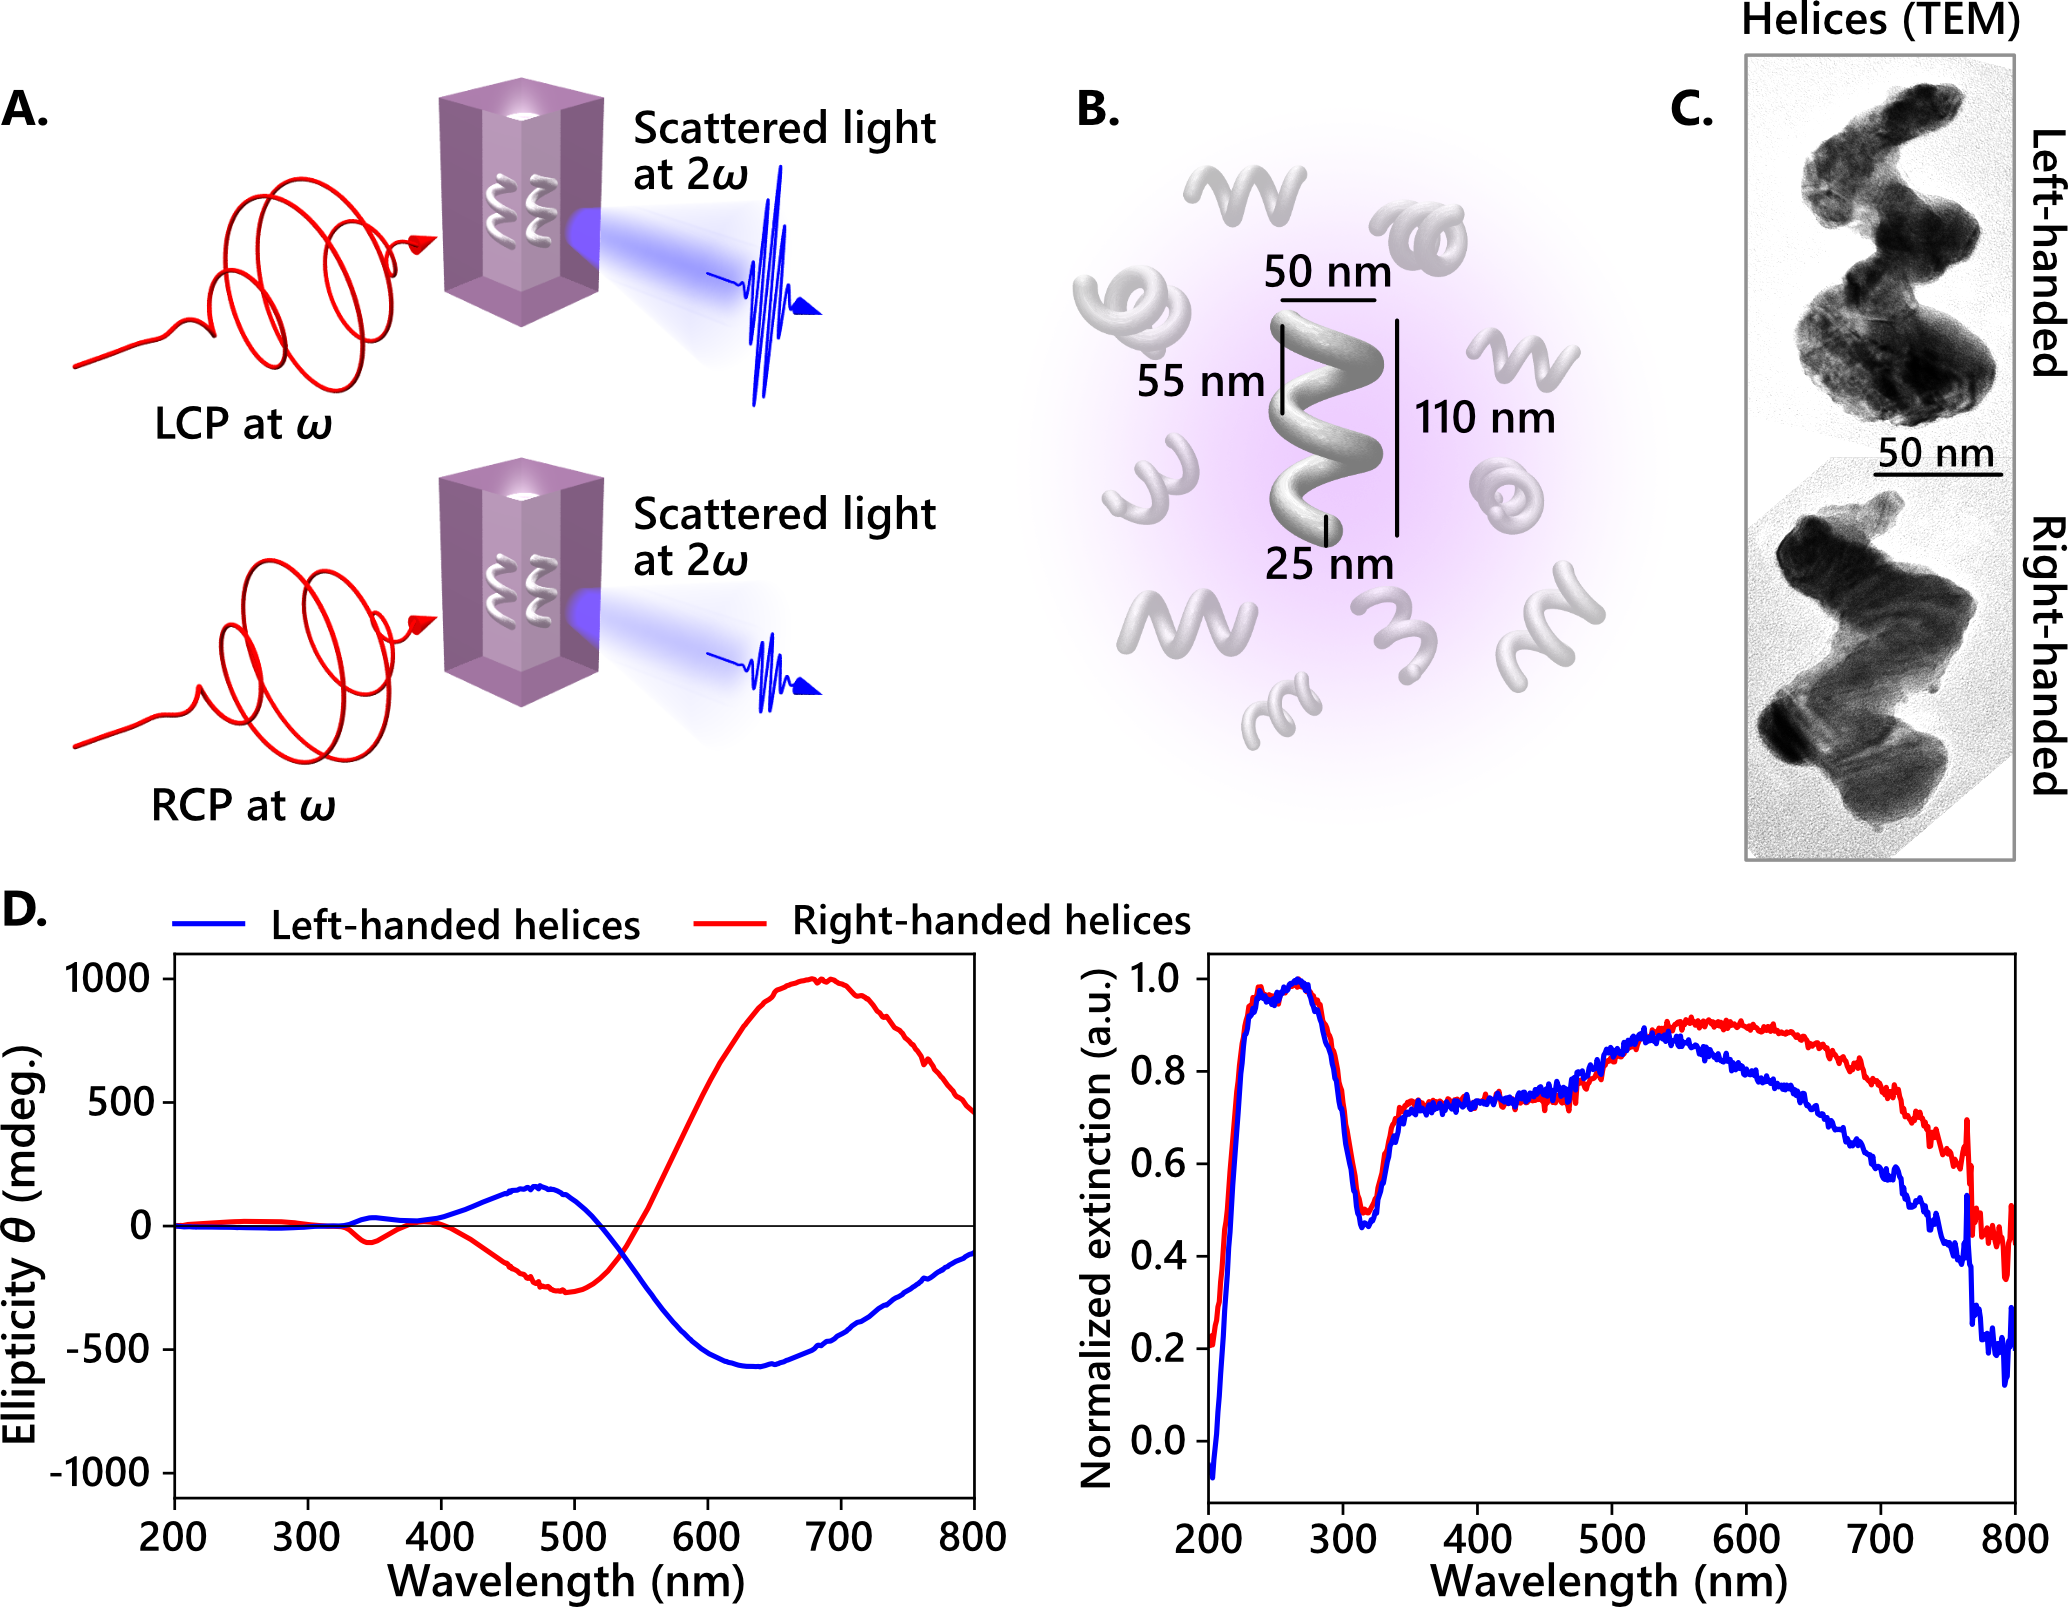
\includegraphics[scale=0.5]{./figures/test_fig_1.png}
    \caption{\label{fig:test_include:test_figure}A little test figure.}
\end{figure}